% background
% brief review of previous research (cite)
% reson why the research was undertaken
% Hypothesis
% explenation of techniques and why they ve been chosen
% objectives = what you hope to achieve
% brief reference to the main outcome

%$\ce{CdS_x Se_{1-x}/ZnS}$

% \begin{figure*}
%   \centering
%   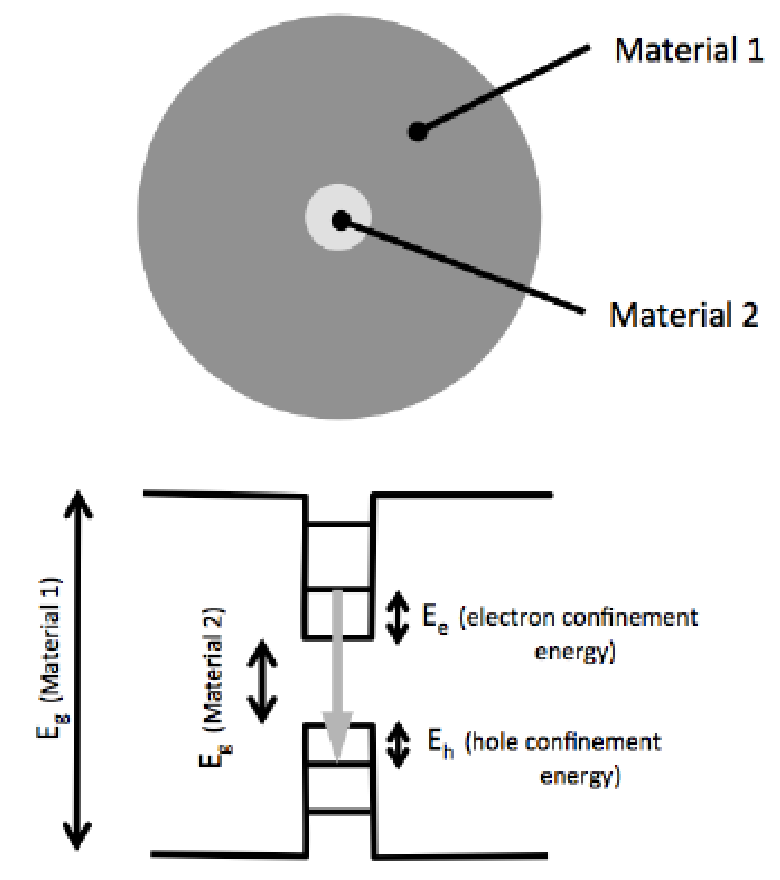
\includegraphics[width=0.35\textwidth]{graphics/QD.png}
%   \caption[width=0.4\textwidth]{\cite{instruction}.}
%   \label{fig:QD}
% \end{figure*}

\section{Introduction}
\label{sec:Introduction}
% Application of low-dimensional organic semiconductors in spintronics
As part of the course "Semiconductors and nanostructures" the aim of this short report is to get a deeper view into a specific subject of the course, such as getting an understanding of the current state of the art research.
Therefore, I want to focus on the application of organic semiconductors in spintronics, their benefits compared to conventional semiconductors and their preparation up to a functioning circuit.
A figure of merit for finding suitable organic semiconductors (OSCs) in the field of spintronics, as well as the spin- and charge propagation are discussed.
The idea of spintronics will be introduced shortly and only in the parts which are used in the example functionality of a spin-OLED, as spintronics itself is an upcoming research field with several different paradigms and branches.
The special behaviour of monocrystalline OSCs is introduced.%, as well as alternative promising materials such as Perovskites.

\section{Spintronics}
\label{sec:spintronics}

The word "spintronics" sets together from the words "spin" and "electronics", and thus means the exploitation of electrons spin instead of its charge for computing.
The most famous example of metal based spintronics in use is the giant magnetoresistance effect (GMR), which is used in hard disk drives.
Here, the resistance of a multilayer device depends strongly on the relative magnetization of two magnetic layers stacked on each other \cite{perovskite}.

In spintronics, information can be stored in a spin state of an electron, which is described by magnetism.
The information can travel by spin-polarized charge or by spin-waves, which are collective oscillations of electrons doing precession motion around a fixed direction of magnetization \cite{clocks}.
Here, the properties of either wave amplitude or phase, or a combination of both can code the information states, as depicted in figure \ref{fig:spin-coding}.

\begin{figure}
  \captionsetup{width=0.9\linewidth}
  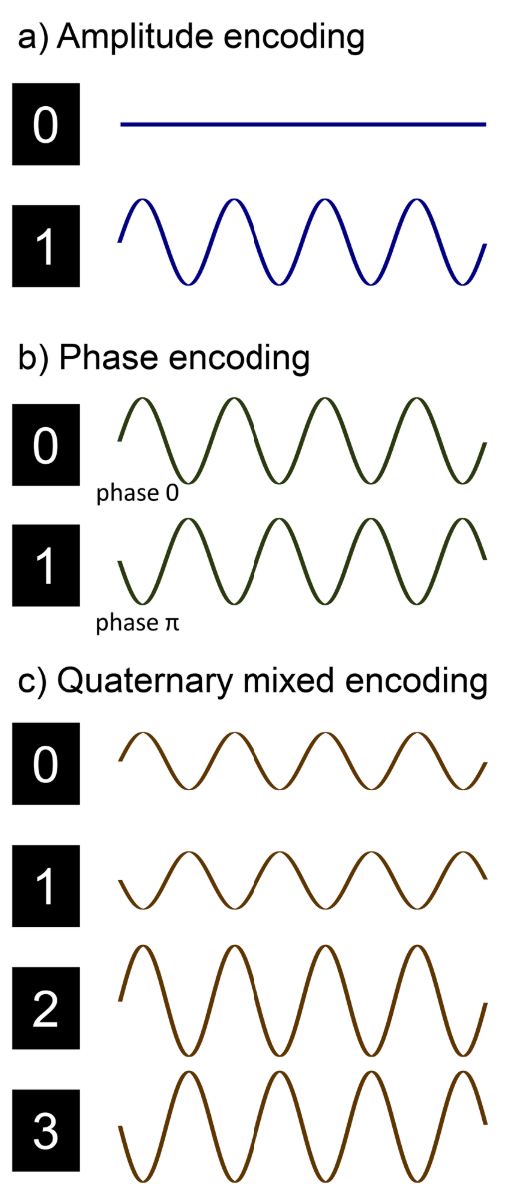
\includegraphics[width=0.4\textwidth]{graphics/spin-code.png}
  \caption{Comparison of schemes to encode information in spin-waves \cite{computing}.}  
  \label{fig:spin-coding}
\end{figure}

In order to process information, unconventional physical interactions have to be considered, such as interference, spin-orbit-coupling and quantum magnetic interactions \cite{perovskite}.

One can see, that easily more than a binary coding system can be introduced. 
Further it is imaginable to use the same device simultaneously for several calculations, as wave properties allow superposition \cite{computing}.

Using spin-waves for information transport gives the opportuntity of low-energy-consumption, non-volatile and less material consuming computing \cite{clocks}. 
In order to built and interconnect a full set of boolean logic circuits to a functioning, complex device, the biggest problem is the small ($\sim\SI{10}{\micro\meter}$ \cite{computing}) propagation, and exponentially decreasing attenuation length of spin waves in metals, which classically may be solved by rather complicated amplification steps (compare \cite{clocks}).

The magnetic damping of the spin wave as well as the group velocity are dependant on the material and geometry of the waveguide \cite{computing} \cite{SC-spintronics}.
Another problem is the interconnection between classical, charge-based circuits and spintronic devices, which bases on magnetic-coupling \cite{clocks}. 
Here, there are different strategies for so called spin-injection \cite{perovskite}, which will be more elaborated in the next chapter about organic spintronics.
To optimate these processes, a good understanding of spin-relaxation and spin-transport mechanisms in metals and semiconductors is the basis, so researchers invested a lot of time in these fields recently \cite{perovskite}.
Further, the impact of dimensionality, defects and the band structure are in big interest \cite{perovskite} \cite{SC-spintronics}.


\section{Organic spintronics}
\label{sec:org-spintronics}
% criteria for material choice and example materials
On the search for spin-waveguides, thus for materials through which a spinwave can propagate long distances without loosing coherence or intensity, organic semiconductors became promising candidates.
In more detail, $\pi$-conjugated organic semiconductors are composed of elements with low atomic number $Z$.
Because the spin-orbit coupling is proportional to $Z^4$ \cite{routes}, which partially is in charge of the spin-wave damping, it is small \cite{appl-organic}.

To get criteria for finding or designing a "good" organic semiconductor for spintronics, a figure of merit is useful.
Regarding the functionality as a waveguide a good spin transport is a indispensable property.

The spin transport can be rationalized by the Einsteins`s relationship 
\begin{equation}
    \lambda_e = \sqrt{(D_\text{hop} + D_\text{ex})\tau_s},
\end{equation}
where $\lambda_s$ is the spin diffusion, $D_\text{hop}$ the diffusion coefficient for hopping mode spin transport (phonon-assisted tunnelling), $D_\text{ex}$ the diffusion coefficient for spin transport following exchange coupling mode and $\tau_s$ is the spin relaxation time \cite{perovskite}.
The exchange coupling, which occurs for high carrier concentration provides faster spin diffusion, as it is decoupled from charge transport.
The Einstein equation is valid also for disordered OSCs except of non-equilibrium conditions such as deep traps, where the states are discharged by recombination.
Nevertheless, the Einstein relationship provides a figure of merit for good spin transportation \cite{single-crystals}.

Therefore, a good charge transport and long spin relaxation time are needed, which are discussed below.

Spin relaxation in a OSC occurs due to spin-orbit coupling, exchange interaction and hyperfine interaction.


%spin relaxation mechanisms
\subsection{Spin relaxation mechanisms}

\begin{figure*}
  \centering
  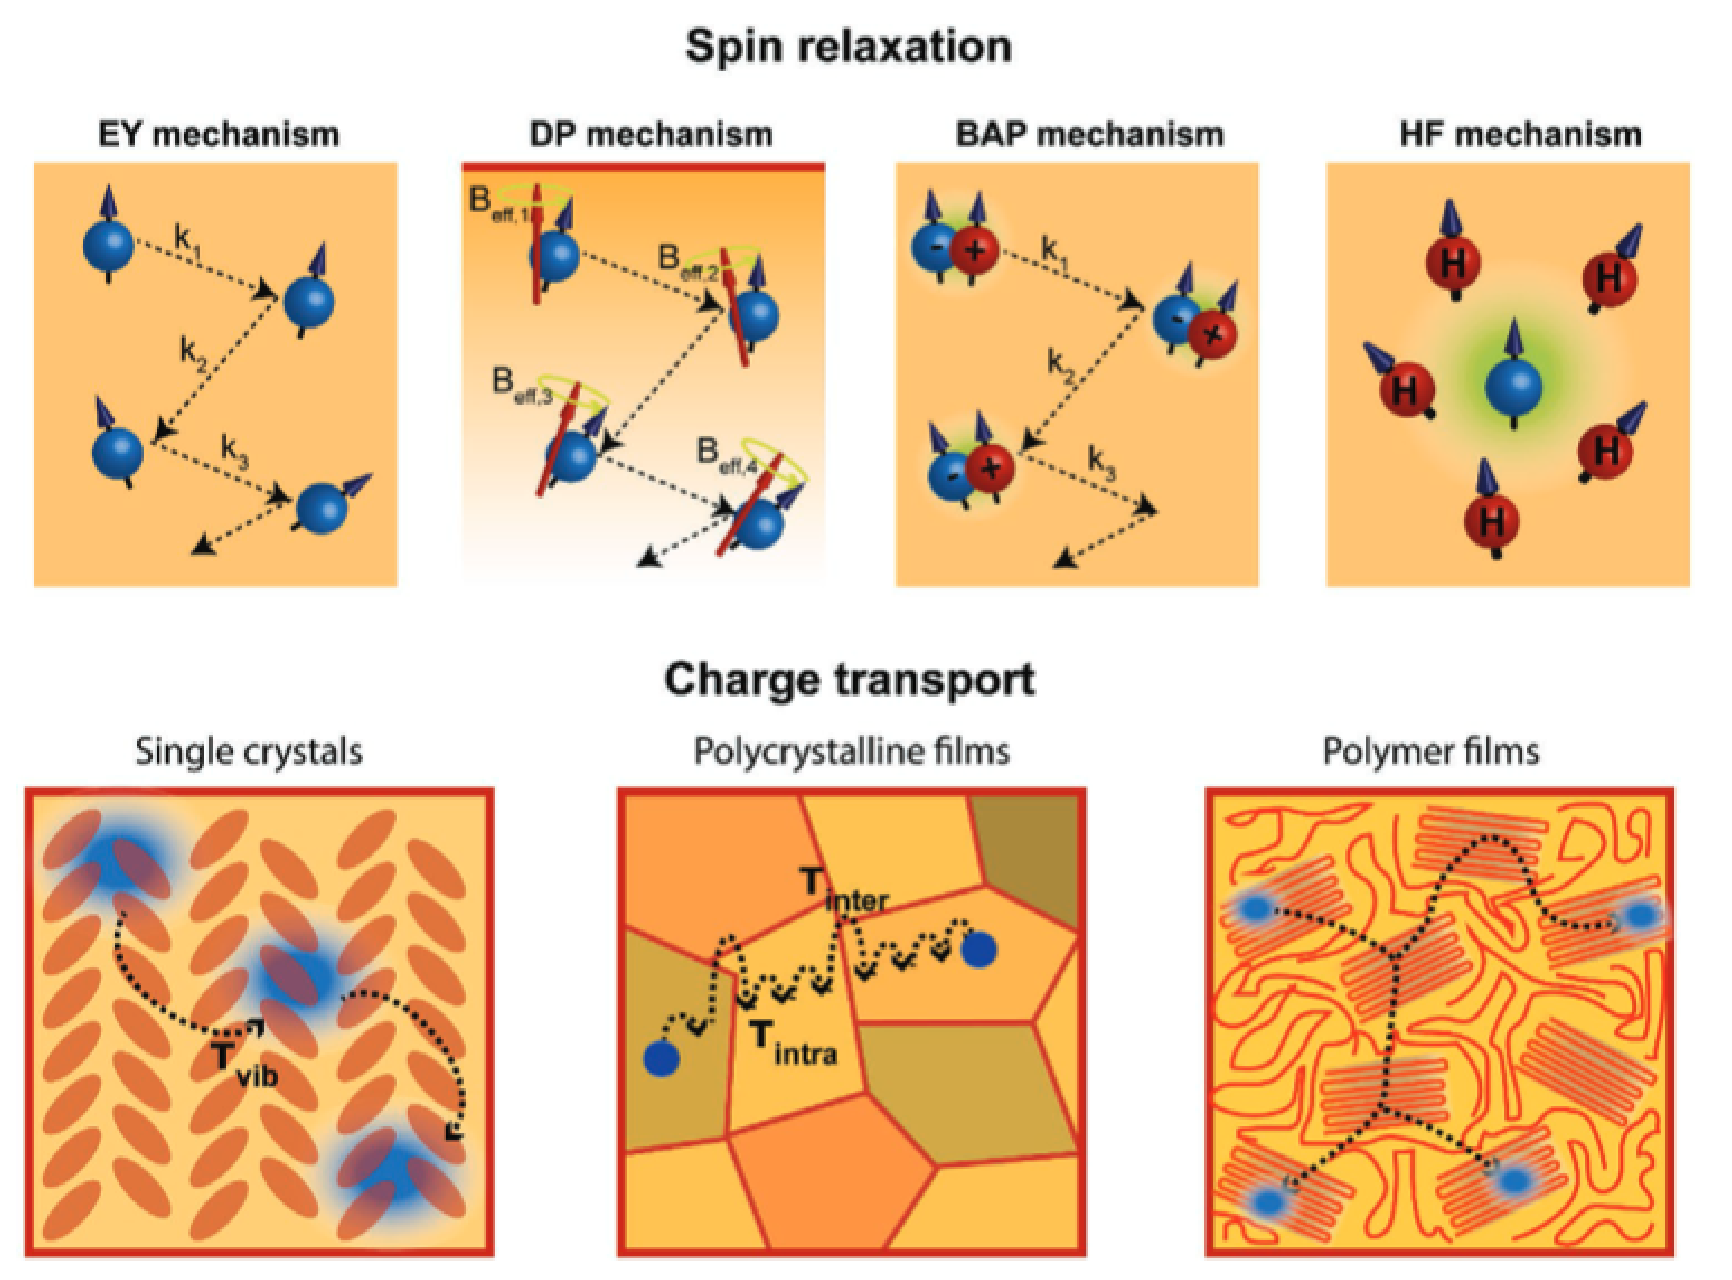
\includegraphics[width=0.7\textwidth]{graphics/relaxation.png}
  \caption[width=0.85\textwidth]{Top: Main four spin relaxation mechanisms occurring in OSCs. From left to right there is the Elliot-Yafet, D`yakonov-Perel, Bir-Aronov-Pikus and hyperfine-effect. Bottom: Charge transport mechanisms from left to right there are single crystals with transient localization of charge carriers, polycrystalline films, where inter-grain transport hinders the fast intramolecular charge transport and polymer films where amorphous regions are the bottleneck of carrier mobility \cite{perovskite}.}
  \label{fig:relaxation}
\end{figure*}

The strongest relaxation mechanism related to spin-orbit coupling is the Elliot-Yafet (EY) mechanism, where momentum scattering of charge carriers also changes the spin orientation due to spin-orbit coupling \cite{elliott}.
As mentioned above, the spin-orbit coupling of OSCs is very small in OSC as these are built up from light, low $Z$ elements.
Experementally, this benefit can be shown by comparing tris-(8-hydroxyquinoline) aluminum ($\ce{Alq_3}$) with tris(2-phenylpyridine) ($\ce{Ir(ppy)_3}$), which has similar chemical structure but different atomic numbers \cite{perovskite} \cite{single-crystals}.

But also the molecular structure has an influence to the spin orbit coupling, which is shown by a measurement done by Yu.
Here, the spin orbit coupling is lower for sexythiophene (t6) and copper phthalocyanine (CuPc) than for $\ce{Alq_3}$ although the aluminum has the lower atomic number.
This behaviour can be explained by a stronger spin-mixing in the $\ce{Alq_3}$ molecule \cite{perovskite}.

The exchange interaction describes the interaction between electrons and conduction band such as holes and the valence band.
It is the basis for the Bir-Aonov-Pikus (BAP) mechanism, which is mainly responsible for the spin relaxation of conduction electrons (valence holes) in p-doped (n-doped) semiconductors.
Here, the electron-hole coupling flips for example the electron if the hole`s spin has been flipped.
This mechanism is especially present in devices like spin OLEDs \cite{perovskite} \cite{spin-OLED}.

The hyperfine (HF) interaction dominates the spin relaxation mechanism for strongly space localized charge carriers as they exist in OSC.
The so called HF mechanism is caused by the effective magnetic field generated by the nuclear spin, which interacts with the electron and thus promotes a spin relaxation.
For the elements relevant in OSCs, the hydrogen atoms H have the biggest nucleus spin, and thus should be overcome.
By replacing H by D, the effective HF interaction can be decreased by a quarter, so that D-based polymer show a longer spin diffusion length \cite{perovskite} \cite{hyperfine}.

%charge transport
%theory of charge transport in OSC
\subsection{Charge transport}

About the spin-dependent charge transport in OSC we know, that it is much more complicated than the band-like transport in non-organic semiconductors.
The delocalized carriers inside the molecules are coupled with weak van-der-Waals interconnections between the molecules, what heavily limits the overall carrier mobility.
The carriers propagate by random, thermally assisted hopping between pseudo-localized states.
In addition, the typical band-like conduction of LUMO and HOMO are taking place inside the molecule and can be spin-polarized.
Defect and interface states may have to be taken into account depending on the materials quality \cite{routes} \cite{perovskite}.
If these are neglectable one speaks from molecular crystals which are discussed further below.

In evaporated thin films of small molecules there are defects and grain boundaries present.
As presented above the limiting factor of charge carrier mobility are the boundaries between the single crystals.
Nevertheless, by morphology control the number of grain borders and their energy barriers can be reduced.
Applied methods are the control of chemical structure, weight of the evaporated molecules and the application of solvent and thermal annealing \cite{morphology}.
Through these parameters grain size and orientation can be manipulated.
Another parameter is the film thickness, where it could be found that thin films of monogeneous amorphous OSCs transport spin much better \cite{appl-organic}.

The third category of charge transport happens in solution processed films of conjugated polymers.
The implementation of rigid, fused-ring copolymers could solve the problem of low carrier mobility at grain borders, when these are implemented in the intercrystallite region.
There, the special electric structure of these polymers allows them to act as a bridge between the single crystals \cite{perovskite}.
Still it is important to notice, that the mismatch of crystal orientation hinders the carriers flow on a long distance range.

% Spin valve measuring
\subsection{Spin valve}

In order to measure the spin transport, a spin valve setup can be used, where the spin-transport layer is sandwiched between two ferromagnetic electrodes, as seen in figure \ref{fig:valve}.
Here, spin-polarised electrons are injected into the OSC thin film and detected from the second electrode \cite{appl-organic}.
By inverting the direction of the external magnetic field, the two electrodes get magnetized parallel (P) or antiparallel (AP).
So, quantitatively the GMR mentioned in chapter \ref{sec:spintronics} can be expressed by the magnetoresistance $\text{MR} = (R_\text{AP}-R_\text{P})/R_\text{AP}$.
The thickness of the tested OSC layer can be considered as the spin transport length \cite{appl-organic}.

In more detail, a reliable spin valve preparation where penetration of metal atoms into the OSC has to be impeded is very important to get reliable data.
This turns out to be a big technical difficulty for thin film fabrication as OSCs are soft materials. 

\begin{figure}
    \centering
  \captionsetup{width=0.9\linewidth}
  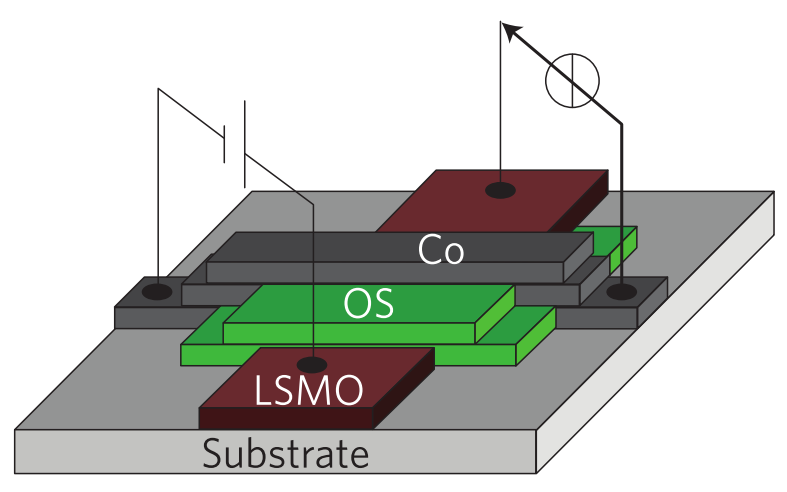
\includegraphics[width=0.4\textwidth]{graphics/valve.png}
  \caption{Spin valve where a OSC (green) is stacked between two ferromagnetic cathodes (LSMO and Copper) \cite{routes}.}
  \label{fig:valve}
\end{figure}

Nevertheless, by using the spin valve it becomes possible to analyse the impact of molecular structure, composition and aggregation structure, which all have vast impact on the spin-transport quality \cite{appl-organic}.

\subsection{OSCs functionalities}

% additional benefits and functionalities
In addition to the good spin-conducting properties, organic semiconductors have a set of unique properties such as flexibility, tailorbility and photo-electric properties \cite{appl-organic}.
These photo-electric function for example can be used to integrate detector or sensor functions directly into a spintronic circuit.
In the setup of a spin-valve the opto-electric functionality can be implemented parallel, in the sense that the magnetic response is independent from the optoelectronic properties, or interactive-type where both properties are coupled.
The application for interactive-type spin valves can be found in multimode storage or sensing.
Here the problem can occur, that material properties which are important for one functionality can hinder important properties according to the spin-transport, such as the magnetoresistance.
Therefore it is important to optimize the spin injection at the electrodes themself \cite{perovskite}.

This gives the rise of electrodes made from organic-based magnets, for example tetracyanoethylene (TCNE).
These help overcoming the common conductivity mismatch between metallic and organic materials.
Summing up, the usage of organic-based magnets allows a fully organic spin-valve design, where TCNE functions as injectors and detectors \cite{perovskite}.

Other interactive functionalities can be spin-light emitting diodes, which are mentioned in more detail in chapter \ref{sec:device}, such as spin photovoltaic.

\section{Molecular crystallin OSCs}
\label{sec:2D}

As the preparation of molecular crystalline OSCs is more complex, thus more energy-consuming or costly, the implementation of these parameters may have physical benefits but hinder an economical use.
Therefore I decided to present them separately in this chapter.

Molecular crystals have, in theory perfect crystal structure and symmetry, thus no defects or grain boundaries which exhibits unique charge and spin transport properties.
Still, the molecular structure and molecular packing have huge impact \cite{single-crystals}.
Although the carrier mobility is high and some transport properties are band-like, electronic states of the carriers in molecular crystals are not spatially fully delocalized Bloch electrons \cite{perovskite}.
To increase the carrier mobility further in such a special situation, the energetic disorder and anisotropy of the band structure should be decreased by modifying the molecules structure and packing \cite{perovskite}.
Here, the herringbone packing is a good example, which is shown in figure \ref{fig:packing}a together with other typical packing of OSC.

\begin{figure}
    \centering
  \captionsetup{width=0.9\linewidth}
  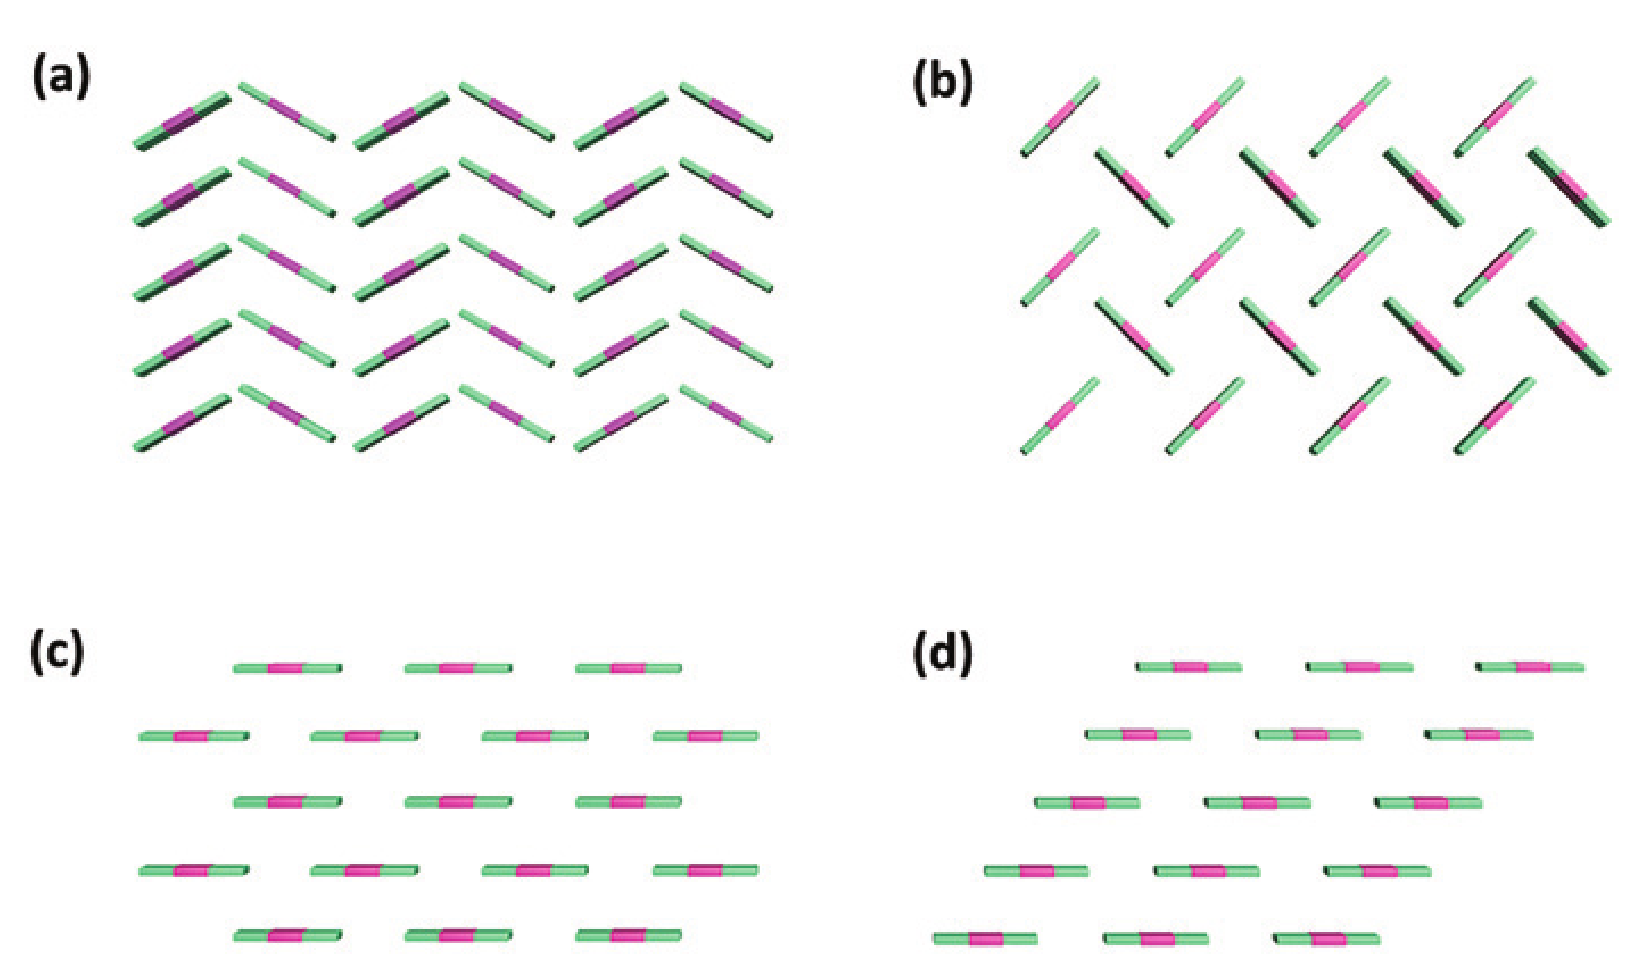
\includegraphics[width=0.4\textwidth]{graphics/packing.png}
  \caption{Common molecular stacking for OSCs with different $\pi - \pi$ overlap: a) herringbone face-to-face b) herringbone edge-face c) brick-wall-stacking with 2D overlap d)slipped stack with 1D overlap \cite{single-crystals}.}
  \label{fig:packing}
\end{figure}

Although here a high carrier mobility and long spin coherence length up to micrometers \cite{single-crystals} could be obtained, some drawbacks are in the production.
The evaporation of the magnetic electrodes needs a lot of temperature which may damage the organic surface \cite{perovskite} \cite{single-crystals}.
A solution can be to use a buffer layer or nitrogen cooling methods \cite{perovskite}.

A here not used, but important technique of producing contacts without damaging the OSC surface is "Layer-sticking", where the cathode is deposited onto the OSC by e mechanical probe. 
This method has also the benefit of avoiding heaking of single metal atoms into the OSC \cite{single-crystals}.


\section{Spin-OLED}
\label{sec:device}
A lot of organic based spintronics devices do still exist only in concept.
They can be divided into two classes which are magnetic resonant tunnel structures or bipolar magnetic diodes and transistors \cite{SC-spintronics}.

An example for a diode based, OSC device are spin-OLEDs, here based on $\ce{Alq_3}$.
The electroluminescent property of OSCs has been used already in conventional OLEDs.
The purpose is to increase the luminous efficienty which can be done by efficient spin injection from magnetic electrodes such as these presented above.
The before mentioned substitution of H by D has been used here, in order to weak the HY interaction in the (H-DOO-PPV) active layer \cite{appl-organic}.
Also, a buffer layer between the organic active layer of Lif and the electrodes has been introduced by Nguyen, to improve the injection efficiency \cite{spin-OLED}.
As seen schematically in the spin-OLED device layout proposed by Prieto-Ruiz, a light-emitting conjugated polymer poly(9,9-dioctylfluorene-co-benzothidiazole) (F8BT) is used.
This one has a high intensity for green light.
A functionality of the device have been proven experimentally for a high bias voltage of 14 V at below room temperature \cite{appl-organic},
so that the current and electroluminescence are both controllable by an external magnetic field \cite{single-crystals}.

\begin{figure}
    \centering
  \captionsetup{width=0.9\linewidth}
  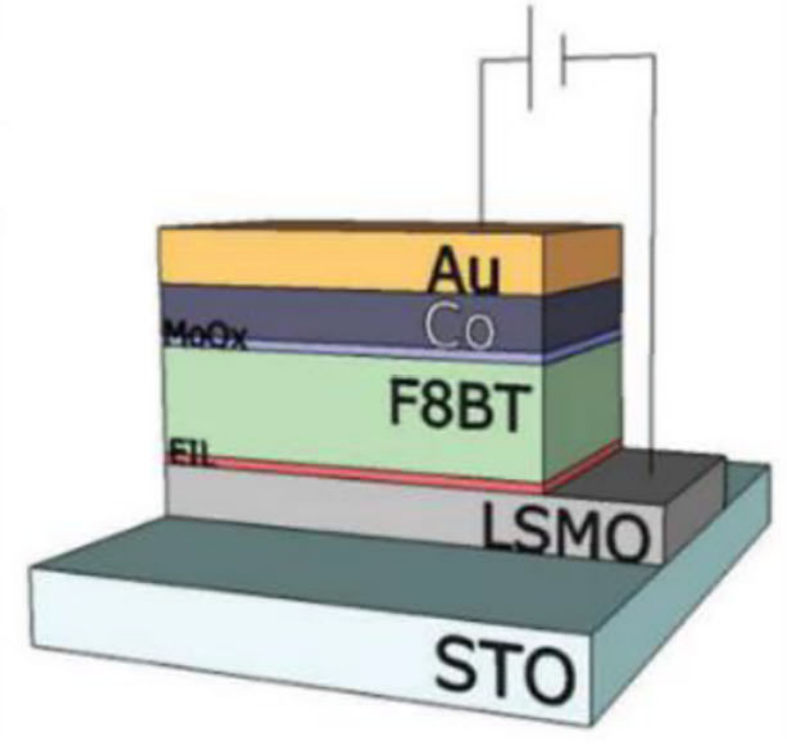
\includegraphics[width=0.4\textwidth]{graphics/oled.png}
  \caption{Schematic structure of a spin-OLED device proposed by Prieto-Ruiz et al. 2019 \cite{appl-organic}.}
  \label{fig:oled}
\end{figure}

% Architecture and manufacturing
% other possible devices

% \section{Alternative materials}
% \label{sec:alternative}
% Perovskites


